%%%%%%%%%%%%%%%%%%%%%%%%%%%%%%%%%%%%%%%%%%%%%%%%%%%%%%%%%%%%%%%%%%%%%%%%%%%%%%%
%                         File: osa-revtex4-1.tex                             %
%                        Date: April 15, 2013                                 %
%                                                                             %
%                              BETA VERSION!                                  %
%                   JOSA A, JOSA B, Applied Optics, Optics Letters            %
%                                                                             %
%            This file requires the substyle file osajnl4-1.rtx,              %
%                   running under REVTeX 4.1 and LaTeX 2e                     %
%                                                                             %
%                   USE THE FOLLOWING REVTeX 4-1 OPTIONS:                     %
% \documentclass[osajnl,twocolumn,showpacs,superscriptaddress,10pt]{revtex4-1}%
%                    %% Use 11pt for Applied Optics                           %
%                                                                             %
%               (c) 2013 The Optical Society of America                       %
%                                                                             %
%%%%%%%%%%%%%%%%%%%%%%%%%%%%%%%%%%%%%%%%%%%%%%%%%%%%%%%%%%%%%%%%%%%%%%%%%%%%%%%

\documentclass[osajnl,twocolumn,showpacs,superscriptaddress,10pt]{revtex4-1} %% use 10pt for Applied Optics
%%\documentclass[osajnl,preprint,showpacs,superscriptaddress,12pt]{revtex4-1} %% use 12pt for preprint option
\usepackage{amsmath,amssymb,graphicx,float,enumerate}
\usepackage[cache=false]{minted}
\usepackage[utf8]{inputenc}
\graphicspath{ {../images/} }

\usepackage{silence}
\WarningFilter{revtex4-1}{Repair the float}

\begin{document}

\title{Redes y Comunicaciones}

\author{Ulises Jeremias Cornejo Fandos}
\affiliation{13566/7, Licenciatura en Informatica, Facultad de Informatica, UNLP}

\author{Federico Ramón Gasquez}
\affiliation{13598/6, Licenciatura en Informatica, Facultad de Informatica, UNLP}

\author{Lihuel Tierni Amoroso}
\affiliation{12345/0, Analista en TIC, Facultad de Derecho y Ciencias Juridicas, UNLP}

%%\begin{abstract}
%%\end{abstract}

\maketitle %% required

\onecolumngrid

\section{Ejercicio 1}

Descargue la captura .pcap del servidor \textbf{http://redes.catedras.linti.unlp.edu.ar/smtp/smtp.pcap} Para ello la petición GET deberá contener el header \textit{x-custom-redes2018}. \\

Para descargar el archivo \textit{.pcap} se utiliza el comando curl ejecutando los siguientes comandos en la terminal.

\begin{minted}{bash}
  $ URL=http://redes.catedras.linti.unlp.edu.ar/smtp/smtp.pcap
  $ curl -H "x-custom-redes2018: value" $URL --output smtp.pcap
\end{minted}

\section{Ejercicio 2}

Extraiga de la consulta .pcap descargada las consultas DNS y los datos correspondientes a SMTP. \\

\section{Ejercicio 3}

Analizar consultas DNS realizadas por el servidor SMTP origen.

\begin{figure}[H]
    \centering
    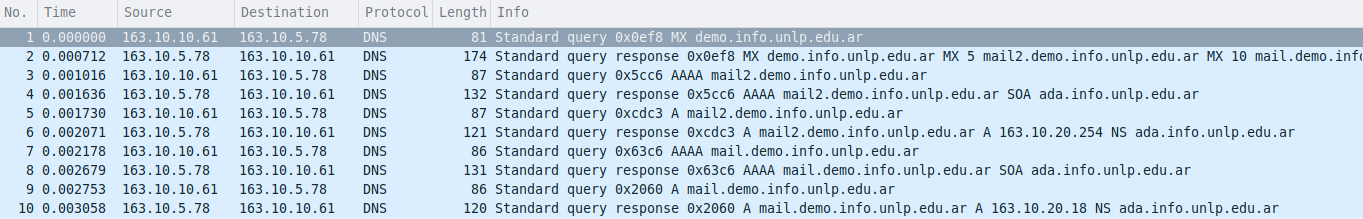
\includegraphics[width=1.0\textwidth]{dns}
    \caption{Consultas DNS realizadas por el servidor SMTP origen.}
\end{figure}

\begin{enumerate}[a)]
  \item ¿Cuál es el servidor DNS recursivo que utiliza el servidor SMTP origen? \\

  Mirando la primer consulta DNS realizada, podemos observar que el servidor DNS recursivo al cual hace la consulta tiene como IP 163.10.5.78. \\

  \item ¿Cuáles son las consultas DNS que realiza? \\

  Las consultas DNS realizadas son las siguientes:

  \begin{enumerate}[1.]
    \item Primero se hace una consulta DNS al servidor con IP 163.10.5.78 para obtener el servidor de mail de `demo.demo.info.unlp.edu.ar` haciendo una consulta DNS de tipo MX.

    En la respuesta de la misma se obtienen los datos de dos servidores de mail. Los mismos son `mail2.demo.info.unlp.edu.ar` y `mail.demo.info.unlp.edu.ar` con preferencias 5 y 10 respectivamente. \\

    \item Posteriormente, se pide conocer la IP del servidor de mail con mayor nivel de preferencia, 5. Entonces se hace una consulta DNS de tipo AAAA al mismo servidor que en el caso anterior para conocer la IPv6 del servidor de mail `mail2.demo.info.unlp.edu.ar`.

    Dado que la respuesta de la consulta es vacia y no existe ningun error en la conexión, podemos saber que el mismo no tiene una IPv6 asociada. \\

    \item Se procede a consultar por la IPv4 del servidor `mail2.demo.info.unlp.edu.ar` haciendo una consulta DNS de tipo A. En la respuesta de la consulta podemos ver que se obtiene la ip 163.10.20.254. \\

    \item Posteriormente, se pide conocer la IP del servidor de mail con nivel de preferencia 10. Entonces se hace una consulta DNS de tipo AAAA al mismo servidor que en el caso anterior para conocer la IPv6 del servidor de mail `mail.demo.info.unlp.edu.ar`.

    Dado que la respuesta de la consulta es vacia y no existe ningun error en la conexión, podemos saber que el mismo no tiene una IPv6 asociada. \\

    \item Se procede a consultar por la IPv4 del servidor `mail.demo.info.unlp.edu.ar` haciendo una consulta DNS de tipo A. En la respuesta de la consulta podemos ver que se obtiene la ip 163.10.20.18. \\
  \end{enumerate}

  \item ¿Alguna de las respuestas es de tipo autoritativa? \\

  Mirando el flag \textit{Authoritative} de las respuestas a cada una de las consultas podemos ver que ninguna de ellas son de tipo autoritativo. \\
\end{enumerate}

\section{Ejercicio 4}

Análisis de SMTP

\begin{enumerate}[a)]
  \item ¿A qué servidor SMTP se conecta el servidor de correo origen? ¿Por qué? \\

  Observando la primer fila de los datos correspondientes a SMTP podemos ver que el servidor de mail con el que se logra establecer la conexión tiene ipv4 163.10.20.18, es decir, que se conecta con el servidor `mail.demo.info.unlp.edu.ar`. \\

  \item ¿Cuántas comunicaciones SMTP se observan en la captura? \\

  Se observan dos comunicaciones SMTP. \\
\end{enumerate}

\section{Ejercicio 5}

Sobre el primer correo electrónico \\

\begin{enumerate}[a)]
  \item ¿A qué corresponde la información enviada por el servidor destino como respuesta al comando EHLO? Elija dos de las opciones del listado e investigue la funcionalidad de la misma. \\

  La información que envia el servidor como respuesta al EHLO es:

  \begin{itemize}
    \item mail
    \item PIPELINING
    \item SIZE 10240000
    \item VRFY
    \item ETRN
    \item STARTTLS
    \item AUTH PLAIN LOGIN
    \item AUTH=PLAIN LOGIN
    \item ENHANCEDSTATUSCODES
    \item 8BITTIME
    \item DSN
    \item SMTPUTF8
  \end{itemize}

  \item ¿Por qué el contenido del primer mail no puede ser leído? \\

  Se envia el mail de forma segura utilizando TLS. \\
\end{enumerate}

\section{Ejercicio 6}

Con respecto al segundo correo electrónico \\

\begin{enumerate}[a)]
  \item ¿Cuál es el nombre del servidor de correo origen? \\

  El primer comando que necesitamos enviar al servidor de correo es EHLO o HELO. Este es un saludo básico que inicia la comunicación entre el cliente de telnet y el servidor SMTP. También se pasa el DNS PTR para la dirección IP desde la que nos conectamos, como se determinó previamente. \\

  Luego, el nombre del servidor de correo origen es `mail.linti.unlp.edu.ar` y lo sabemos dado que se envia como parámetro del comando EHLO. \\

  \item ¿Cuál es el MESSAGE-ID del correo enviado? ¿Quién asigna dicho valor? \\

  En la fila 20 de los datos filtrados para el protocolo SMTP, paquete nro. 113 del total de los paquetes del .pcap, se puede ver en el campo Internet Message Format el MESSAGE-ID del mail enviado y este es:
  
  \textit{$<$94c3492a-4bf1-c0c8-c059-c2cb2216d2f8@linti.unlp.edu.ar$>$} \\
  
  \item ¿Cuál es el producto que implementa el servidor de correo origen y cuál el destino? \\
  
  

\end{enumerate}



\end{document}
